\documentclass[a4paper]{article}

\usepackage[english]{babel}
\usepackage[utf8]{inputenc}
\usepackage{amsmath}
\usepackage{graphicx}
\usepackage{listings}
\lstset{language=Pascal}
\usepackage[colorinlistoftodos]{todonotes}

\title{Machine Learning Stanford}

\author{Dylan Bourgeois}

\date{\today}

\begin{document}
\maketitle

\begin{abstract}
Notes from Coursera class.
\end{abstract}

\section{Introduction}

Introduction to Machine Learning.

Supervised : give the right answer. Regression predicts real value output.

\section{Model}
\label{sec:examples}

\subsection{Model Representations}

Training set = data set. \textbf{m} = number of training examples.

Training set $\to $ Learning algorithm $\to h(x)=y$. 

\textbf{h} is the \textit{hypothesis}, a linear function that outputs results for given entry x. 
$$h(x) = \theta_0 + \theta_1.x $$  
Linear regression with one variable == Univariate linear regression. 

\subsection{Cost Function}

We must minimize the cost function (also called \textit{squared error function}), which is function of $\theta_0$ and $\theta_1$.
$$J(\theta_0, \theta_1) = \frac{1}{2m}\sum_{i}^{m} (h_\theta (x_i)-y_i)^2$$

\subsection{Cost Function Intuition}

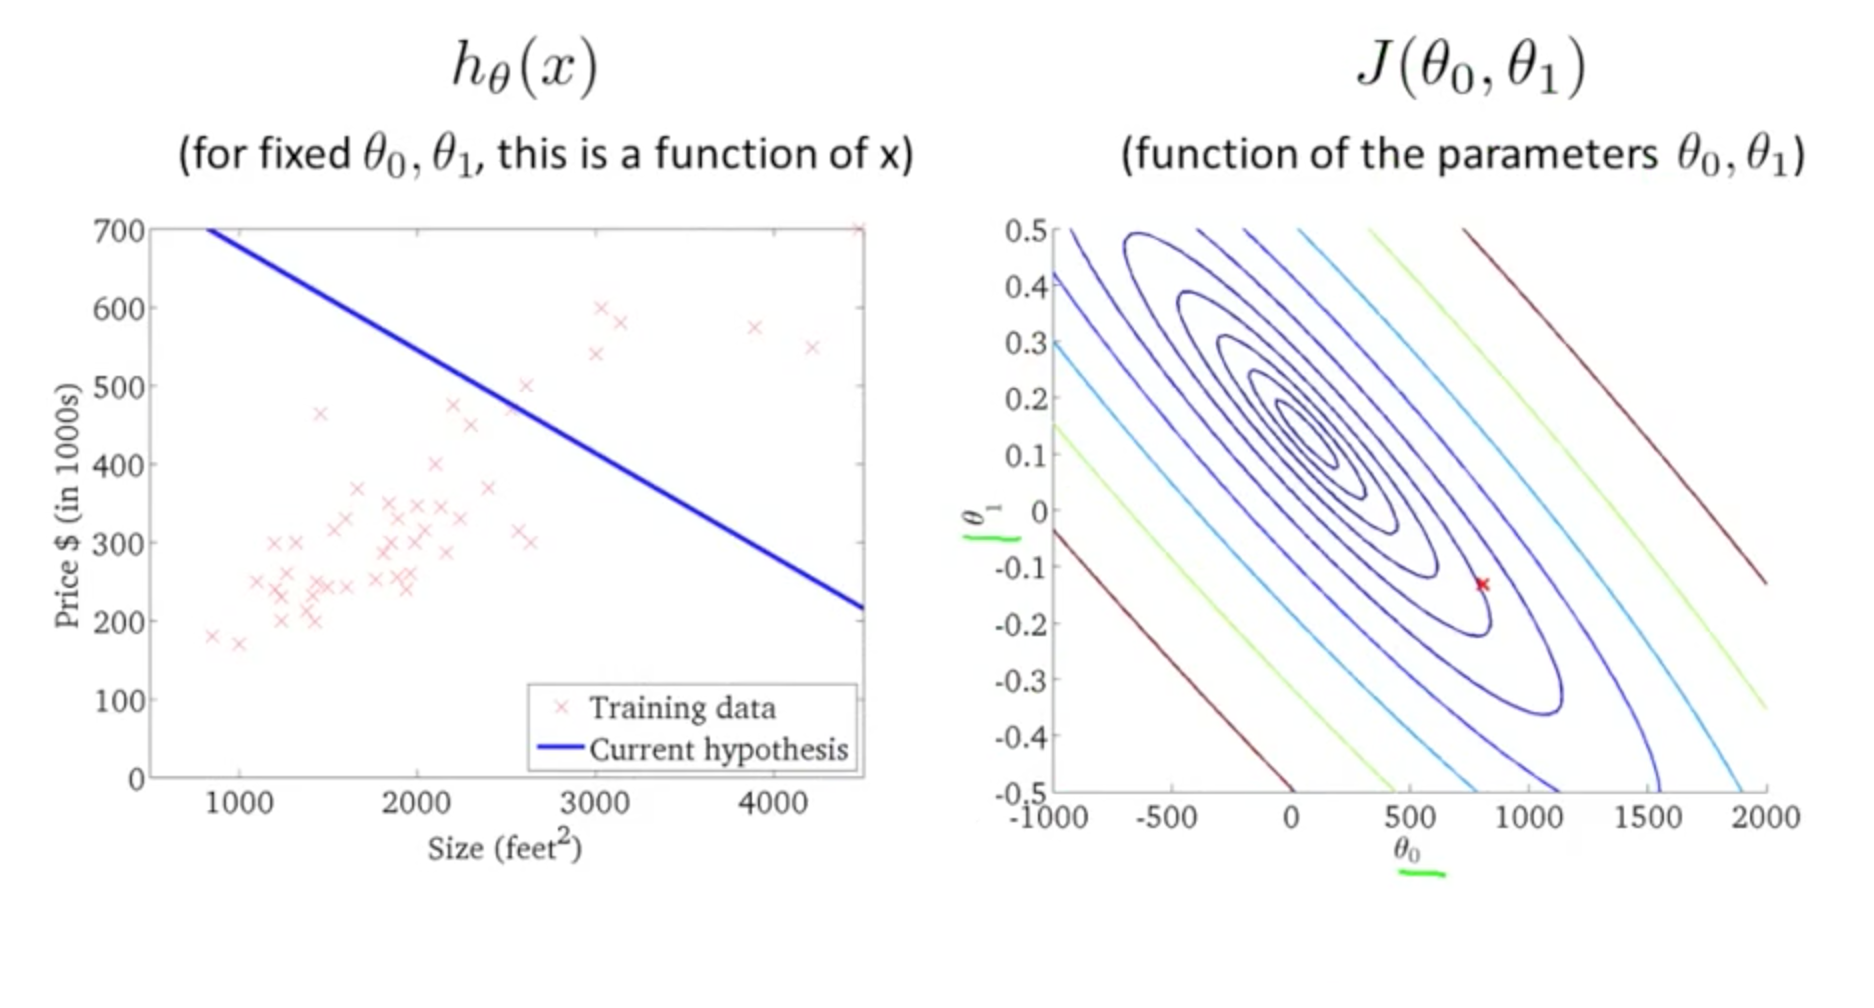
\includegraphics[scale=0.35]{MLS.png}

For linear regression, the contour plot of the cost function is a series of concentruc ellipses. The center of these ellipses is the minimum of this function, so is the point for the desired $(\theta_0, \theta_1)$ tuple.

\subsection{Gradient Descent}

This method is valid for $n$ parameters, so for $J(\theta_0, \ldots ,\theta_n)$.
Start with a given tuple $(\theta_0, \theta_1)$, and update the value \textbf{simultaneously} until covergence :
$$\theta_j := \theta_j - \alpha \frac{\partial J(\theta_0,\theta_1)}{\partial \theta_j}   \quad for j=0,1;\quad \alpha = learning \, rate $$

We must assign the new values \textbf{simultaneously} : 
\begin{lstlisting}[frame=single]
until Gradient Descent converges do
begin
{ 
    tmp0 = theta0 - alpha * d(J)/dtheta0;
    tmp1 = theta1 - alpha * d(J)/dtheta1;
    theta0 = tmp0;
    theta1 = tmp1;
}
end;
\end{lstlisting}

\subsection{Gradient Descent Intuition}

If $\alpha$ is small, gradient descent can be slow. If $\alpha$ is too large, gradient descent can overshoot the minimum. It may fail to converge or even diverge. 

If your initial tuple $(\theta_0, \theta_1)$ is already at a local minimum, the gradient descent algorithm will stay at value $\theta_1$. 

As we approach a local minimum the gradient descent algorithm will automatically take smaller steps.

\subsection{Gradient descent for linear regression}
 Also called catch gradient descent algorithm: on each step you are looking at all the training examples. We need to calculate the derivative of $J(\theta_0,\theta_1)$ for 
$$j = 0 \quad \frac{1}{m} \sum_{1}^{m} h(x_i)-y_i $$ 
$$j = 1 \quad \frac{1}{m} \sum_{1}^{m} x_i(h(xi)-yi)$$ 
For linear regression, $J(\theta_0,\theta_1)$ is a convex function, which has only one global minimum : no other local minimum than the global minimum.

\end{document}